\documentclass[12pt,letterpaper,noanswers]{exam}
\usepackage[usenames,dvipsnames,svgnames,table]{xcolor}
\usepackage[margin=0.9in]{geometry}
\renewcommand{\familydefault}{\sfdefault}
\usepackage{multicol}
\pagestyle{head}
\header{AM 108 Fall 2020}{Updated \today.}{Skill List for Skill Checks}
\runningheadrule
\headrule
\usepackage{graphicx} % more modern
\usepackage{amsmath} 
\usepackage{amssymb} 
\usepackage{hyperref}
\usepackage{tcolorbox}

\begin{document}
 \pdfpageheight 11in 
  \pdfpagewidth 8.5in

This document list 27 skills associated with content of the course.  A maximum of one skill is assigned per class meeting.  Skills are drawn from techniques and concepts that are either central to the course or that were challenging for students on past assessments.

\tableofcontents
  
\section{1d systems}
\subsection{find fixed points}
\subsubsection{Question}

 Let $\displaystyle\dot{x} = 4x^2 - 16$.  Use \textbf{linear stability analysis} to find the fixed points and to identify their stability.  \emph{Do not use a graphical approach for this skill check.} %Find the fixed points algebraically.  At each fixed point, compute the slope of the vector field.  Use the slope to identify the stability of each fixed point.

\subsubsection{Solution}
\begin{enumerate}
\itemsep-0.3em
    \item Set $\dot{x} = 0$ to identify fixed points.
    \item Work out the algebra: $4x^2 - 16 = 0 \Rightarrow x^2 = 4 \Rightarrow x = -2, 2$.  The fixed points are at $x = -2$ and $x = 2$.
    \item Use the slope of $f(x)$ for the stability.  
    \item Find the derivative with respect to $x$: $\dfrac{df}{dx} = 8x$.
    \item Evaluate the slope at the fixed points: $\left.f'(x)\right\vert_{-2} = -16$ and $\left.f'(x)\right\vert_{2} = 16$.
    \item Use the sign of the slope to identify the stability of the fixed point: negative slope means $\dot x > 0$ to the left of the fixed point ($x(t)$ is increasing) and $\dot x < 0$ to the right of the fixed point ($x(t)$ is decreasing).  $x = -2$ is a stable fixed point.  $x = 2$ is an unstable fixed point.
\end{enumerate}


\subsection{recognize bifurcations}

\subsubsection{Question}
For each of the four bifurcation diagrams given below, name the bifurcation that occurs in the diagram.

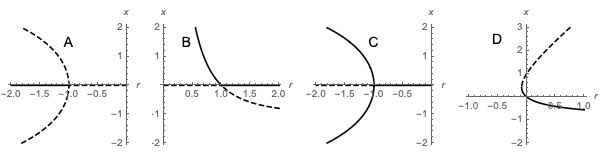
\includegraphics[width=\linewidth]{img/C04-2019-09-11bifn.png}


\bgroup
\def\arraystretch{2}
\begin{tabular}{|l|p{10cm}|}
\hline
Plot     & \hspace{0.5cm} Bifurcation name \\
\hline\hline
 A    & \\
 \hline
 B & \\
 \hline
 C & \\
 \hline
 D & \\
 \hline
\end{tabular}
\egroup

\subsubsection{Solution} 

The possibilities are: saddle-node bifurcation, transcritical bifurcation, supercritical pitchfork bifurcation, subcritical pitchfork bifurcation.  There are all the bifurcations we have learned so far.

In (A) the bifurcation point is at $r = -1$.  Very close to the bifurcation there are three branches to one side and one to the other side.  The $x=0$ fixed point changes stability at the bifurcation and the two extra branches are both unstable.  This is a \emph{subcritical pitchfork bifurcation}.  (Subcritical because the extra branches are unstable).

In (B) the bifurcation point is at $r = 1$.  Very close to the bifurcation there are two branches to each side, so it is a \emph{transcritical bifurcation}.

In (C) the bifurcation point is at $r = -1$.  Very close to the bifurcation there are three branches to one side and one to the other side.  The $x=0$ fixed point changes stability at the bifurcation and the two extra branches are both stable.  This is a \emph{supercritical pitchfork bifurcation}.  (Supercritical because the extra branches are stable).

In (D) the bifurcation point is at $r$ a little less than $0$.  Very close to the bifurcation there are two branches on one side and no fixed points on the other side.  This is a \emph{saddle node bifurcation}.


\subsection{find dimensionless groups}
\subsubsection{Question}


Consider the differential equation \[\frac{dx}{d\tau} = r T_0\left(\frac{1}{h_v}+ x\right)- \frac{r T_0 A}{K} x.\]
Assume that $x$ and $\tau$ are nondimensional variables and that $r, T_0, A, K$ are parameters with dimension.

Identify two nondimensional groups from the equation above.


\subsubsection{Solution}


 $x$ and $\tau$ are nondimensional.  In addition, quantities that are added to each other or are equal to each other must have the same dimensions.

We have $\left[\dfrac{dx}{d\tau}\right] = \left[r T_0\left(\dfrac{1}{h_v}+ x\right)\right] = \left[\dfrac{r T_0 A}{K} x\right]$ (where $\left[ . \right]$ denotes ``the dimensions of'').

We have $\left[x \right] = \left[\tau\right] = 1$.  So $\left[\dfrac{dx}{d\tau}\right] = 1$ (these are all dimensionless).

The dimension of a product is the product of the dimensions, so

$1 = \left[r T_0\right]\left[\left(\dfrac{1}{h_v}+ x\right)\right] = \left[\dfrac{r T_0 A}{K}\right]\left[ x\right]$.

The dimension of a sum is the dimension of either component of the sum, so

$1 = \left[r T_0\right]\left[x\right] = \left[\dfrac{r T_0 A}{K}\right]\left[ x\right]$.

Using $\left[x \right] = 1$, this is $1 = \left[r T_0\right] = \left[\dfrac{r T_0 A}{K}\right]$.

$rT_0$ is a dimensionless group.  $1 = \left[\dfrac{r T_0 A}{K}\right] = \left[rT_0\right]\left[\dfrac{A}{K}\right]$.  $\dfrac{A}{K}$ is another dimensionless group.  $h_v$ is a dimensionless parameter (but is not a group).

\subsection{identify long term behavior: phase difference}
\subsubsection{Question}

Assume the time evolution of the phase difference, $\phi$, between an oscillator and a reference signal is given by the system $\dot\phi = 1.1-\sin\phi$.

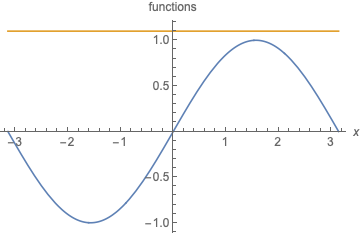
\includegraphics[width=4in]{img/C07-2019-09-18plot2.png}

What is the long term behavior of the phase difference in this system?


\subsubsection{Solution}

 Note that this question requires us to interpret $\phi$ as a phase difference, rather than as the phase of a single oscillator.

If there were an intersection between the orange line and the blue line then the phase difference would approach a fixed value (that you could identify) associated with a stable or half-stable fixed point.

In this picture, though, $\dot\phi = 1.1 - \sin\phi$ and $\sin\phi < 1.1$ for all values of $\phi$.  So $\dot\phi > 0$ for all phase differences, $\phi$.  This means that \textbf{the phase difference is always changing}.  In some sense, it is always increasing ($\dot\phi>0$, after all).  However, when the phase difference passes through $2\pi n$ for $n$ an integer, the oscillator and the reference momentarily have the same phase angle, so if we look at the two oscillators on a circle, one of them will appear to `lap' the other one over and over again. 


\subsection{plot a function}
\subsubsection{Question}

Plot the function $f(N) = H\dfrac{N^2}{A^2+N^2}$.  

\emph{Label your axes and to include at least one (labeled) tick mark on each axis.}

Your plot should have correct behavior for $N\rightarrow 0$, for $N\rightarrow\infty$, and for an appropriate (and labeled) finite value of $N$.



\subsubsection{Solution}

One way to think of this function is as $f(N) = H \dfrac{(N/A)^2}{1+(N/A)^2}$, where $N/A$ is dimensionless.  Let $ x = N/A$.  

The $N$-axis (horizontal) is naturally measured in increments of $A$.  The vertical in increments of $H$.  

As $x\rightarrow \infty$, we have $\lim_{x\rightarrow \infty} H \dfrac{x}{1+x} = H$.  At $x = N/A = 0$ we have $f(0) = H\frac{0}{1+0} = 0$.  At $x = 1$ so $N = A$ we have $f(A) = H\dfrac{A^2}{2A^2} = H/2$.  

The slope as $N\rightarrow 0$ is given by $\left.f'(x)\right\vert_0 = \left.H(2N)(A^2+N^2)^{-1}-HN^2(2N)(A^2+N^2)^{-2}\right\vert_{N=0} = 0$.  Or, using the binomial expansion to approximate the function near $0$, $f(N)= H(N/A)^2(1+(N/A)^2)^{-1} \approx H(N/A)^2(1 - (N/A)^2 + ...)$ (we have $N/A \ll 1$ when $N$ is close enough to $0$).  And for $N$ close to zero, this is $f(N) \approx HN^2/A^2$ (a parabola).

We're now ready to sketch.  The curve passes through $(0,0)$ and leaves the origin going horizontally (tangent to the $N$-axis).  Close to $0$, $f(N) \approx H \dfrac{N^2}{A^2}$, so it will specifically leave the origin with a parabolic shape.  It passes through $f(A) = H/2$ and approaches $H$ as $N \rightarrow\infty$.

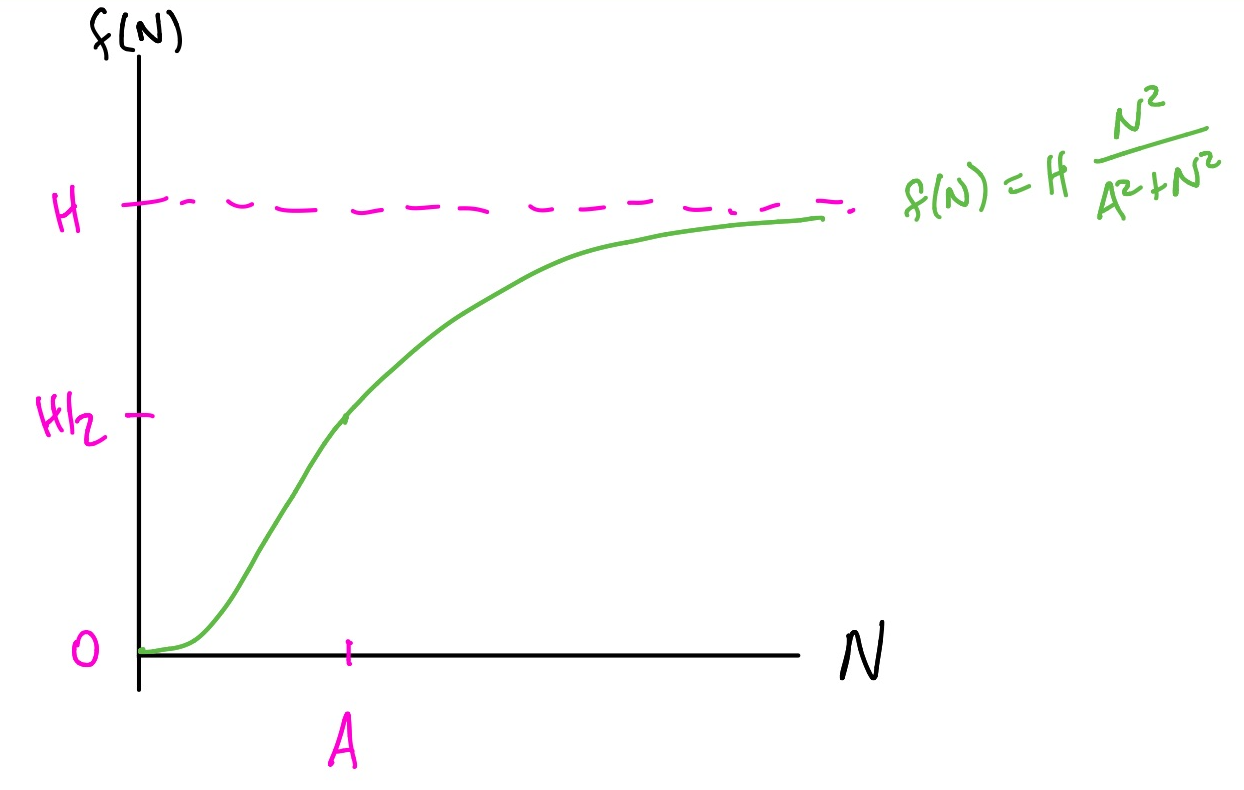
\includegraphics[width=3in]{img/C08soln-Hillfcnplot-p1.png}

\section{2d systems}

\subsection{match a phase portrait and linear system}
\subsubsection{Question}
Consider the 2d linear system $\dot x = 3x+y$, $\dot y = x-y$.  This system can also be written $\displaystyle \frac{d}{dt}\left(\begin{array}{c} x \\ y \end{array}\right) = \left(\begin{array}{c c} 3 & 1 \\ 1  & -1 \end{array}\right)\left(\begin{array}{c} x \\ y \end{array}\right)$.

\[\left(\begin{array}{c} x(t) \\ y(t) \end{array}\right) = 2e^{(1+\sqrt{5})t}\left(\begin{array}{c} 2+\sqrt{5} \\ 1 \end{array}\right)+3e^{(1-\sqrt{5})t}\left(\begin{array}{c} 2-\sqrt{5} \\ 1 \end{array}\right)\] is a solution to this system.

Match this system to its corresponding phase portrait below.

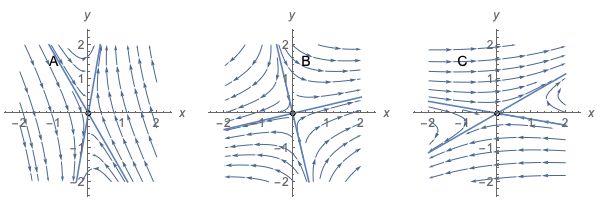
\includegraphics[width=\linewidth]{img/C08prac-2019-09-20.png}


\subsubsection{Solution}
The solution we were given is the weighted sum of an exponentially growing component, and an exponentially decaying one.  Presumably $(2+\sqrt{5},1)^T$ and $(2-\sqrt{5}, 1)^T$ are the eigenvectors of the system.  I'll check that:

$\left(\begin{array}{c c} 3 & 1 \\ 1  & -1 \end{array}\right)\left(\begin{array}{c} 2\pm\sqrt{5} \\ 1 \end{array}\right) = \left(\begin{array}{c} 6 \pm 3\sqrt{5} + 1 \\ 2\pm \sqrt{5} - 1\end{array}\right) = \left(\begin{array}{c} 7 \pm 3\sqrt{5} \\ 1\pm \sqrt{5} \end{array}\right) = (1\pm\sqrt{5})\left(\begin{array}{c} 2\pm\sqrt{5} \\ 1 \end{array}\right)$.

We have an exponentially growing solution $(1+\sqrt{5})\left(\begin{array}{c}2 + \sqrt{5} \\ 1\end{array}\right)$.  This will be a straight line along which trajectories move outward.  For every four units in $x$, we go up one in $y$ along this line.  Based on this, I can eliminate A from the options.

We have an exponentially decaying solution $(1-\sqrt{5})\left(\begin{array}{c}2 - \sqrt{5} \\ 1\end{array}\right)$.  This will be a straight line along which trajectories move towards the origin.  $2 - \sqrt{5}$ is negative but close to zero.  So we move a small distance along the negative $x$ axis for each unit upwards in $y$.  That means the match is B.


\subsection{use trace and determinant to classify a fixed point}
\subsubsection{Question}
Use $\tau$ and $\Delta$ to provide classifications for the following linear systems.  
\begin{parts}
\item Classify each fixed point as either stable (attractors), unstable (repellers or saddle points), or non-hyperbolic (a line or plane of fixed points, or a center). 
\item Identify the type of fixed point(s) (attractor, repeller, saddle point, linear center, line of fixed points, plane of fixed points).  Also specify spiral vs node, if relevant.
\end{parts} 

\begin{tabular}{|c|c|c|c|}
\hline
$\tau$ & $\Delta$ & stable / & attractor, etc/ \\
& & unstable / &  \\
& & non-hyperbolic & \\
\hline
2 & 3 & & \\
&  & & \\
\hline
 1    &  -2& & \\
     & & & \\
     \hline
 0  & 3 & & \\
     & & & \\
     \hline
\end{tabular}

\subsubsection{Solution}
\begin{itemize}
    \item $\tau = 2$, $\Delta = 3$.  $\Delta > 0$ so this is not a saddle point.  $\tau > 0$, so this is a repeller (unstable).  $\tau^2 - 4\Delta = 4 - 12 = -8<0$, so this is a spiral.
    \item $\tau = 1, \Delta = -2$.  $\Delta < 0$ so this is a saddle point, which is an unstable fixed point.
    \item $\tau = 0$, $\Delta = 3$.  $\Delta > 0$ so not a saddle point.  $\tau = 0$ so this is a linear center.  non-hyperbolic (real part of each eigenvalue is zero).
\end{itemize}


\begin{tabular}{|c|c|c|c|}
\hline
$\tau$ & $\Delta$ & stable / & attractor, etc/ \\
& & unstable / &  \\
& & non-hyperbolic & \\
\hline
2 & 3 & unstable & repeller (spiral) \\
&  & & \\
\hline
 1    &  -2& unstable & saddle point\\
     & & & \\
     \hline
 0  & 3 & non-hyperbolic & linear center\\
     & & & \\
     \hline
\end{tabular}

\subsection{use nullclines to identify the direction of flow}
\subsubsection{Question}
For the following nonlinear dynamical system: $\dot x = x(3-x-y), \dot y = y(2-x-y)$, $x,y\geq 0$.
\begin{parts}
\item Sketch the $\dot x = 0$ and $\dot y = 0$ nullclines on the $xy$ phase space.
\item Add a representative vector to each section of the phase space showing direction of the vector field in that region (up and left; up and right; down and left; down and right)
\end{parts} 

\subsubsection{Solution}

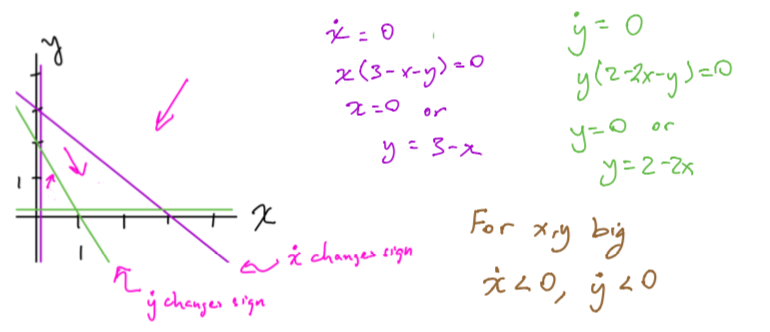
\includegraphics[width=0.9\textwidth]{img/C10-11nullclines-p1.png}


\subsection{finding the derivative of a function along a trajectory}
\subsubsection{Question}
 For the system $\dot x = y, \dot y = x^3-x$, compute $\dfrac{dE}{dt}$ along trajectories for $E =-2 x^2 - 2y^2 + x^4$.

\emph{Show your computational steps}

\subsubsection{Solution}
\begin{enumerate}
\item $E(x,y) = -2x^2 - 2y^2 + x^4.$
\item $\dfrac{dE}{dt} = -4x \dot{x} - 4y\dot{y} + 4x^3\dot x$ (used the chain rule to take the derivative on the right hand side)
\item $\dfrac{dE}{dt} = -4x(y) - 4y(x^3-x) + 4x^3(y)$ (substitute $\dot x = y$ and $\dot y = x^3-x$, as these differential equations are true on trajectories)
\item $\dfrac{dE}{dt} = 0$ (simplify the expression on the right hand side)
\end{enumerate}

\subsection{use a conserved quantity to sketch phase curves}
\subsubsection{Question}
 Let $H(x,y) = xy$ be a conserved quantity for a 2D dynamical system.  Use this information to sketch three phase curves of the system.
 
\subsubsection{Solution}

Phase curves are curves $y=Y(x)$ such that a trajectory that starts on the curve stays on the curve.

Every contour curve $H(x,y) = c$ is such a curve.  Start with $H(x,y) = 0$, so $xy = 0$.  $y = 0$ is a phase curve.  $xy = 1 \Rightarrow y = 1/x$ is another.  $y = 2/x$ is a third.

I'll sketch these three curves in the $xy$-plane.

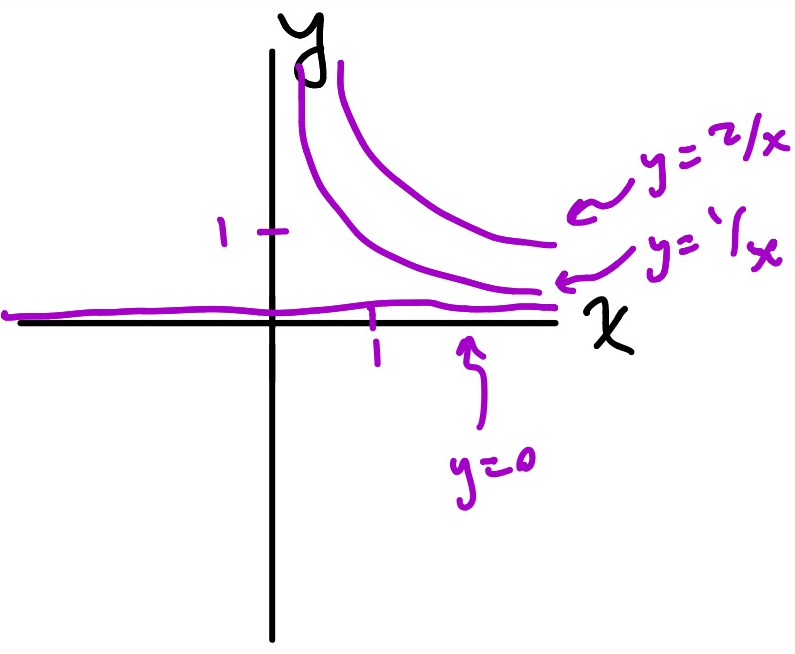
\includegraphics[width=3in]{img/C12curves.png}

\subsection{identify phase portraits that are consistent according to Poincar\'e index theory}
\subsubsection{Question}
According to index theory, is the following phase diagram configuration possible or not?  Briefly support your answer.

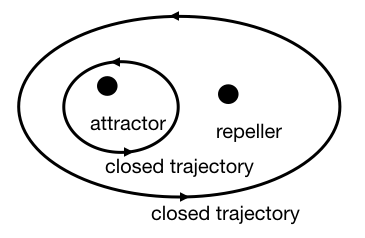
\includegraphics[]{img/C15-2019-10-07p2.png}

\subsubsection{Solution}
Each closed trajectory has an index of $+1$, so needs to enclose fixed points with a total index of $+1$, but the outer one encloses fixed points with a total index of $+2$, so not possible.

\subsection{find a trapping region for a system given in polar}
\subsubsection{Question}
Consider a dynamical system specified by $\dot r = r(2-\sin\theta/2 -r)$, $\dot\theta = 1$, with the phase portrait below.  Use $\dot r$ to identify inequalities that define a trapping region that satisfies the conditions of the Poincar\'e-Bendixson theorem.  Show that you have found a trapping region by identifying the sign of $\dot r$ on the boundary curves of the region.


\emph{The gridlines are drawn with an interval of $1$ units.}


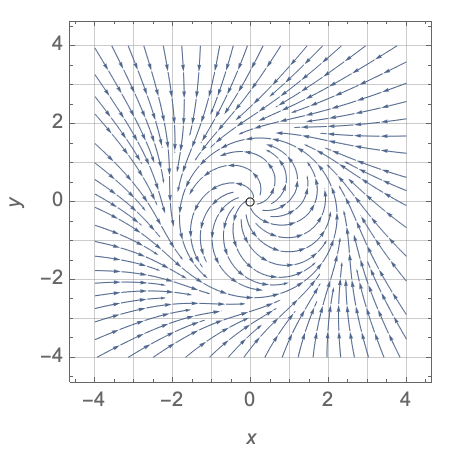
\includegraphics[]{img/C14-C15trapping.png}

\subsubsection{Solution}

We're using polar coordinates for this. $\dot\theta >0$, so there will be no fixed points away from the origin.  I have $\dot r = r(2-\sin\theta/2-r)$.  For $r$ large, $2-\sin\theta/2 -r < 0$.  Specifically, $2-\sin\theta/2$ has a max of $2.5$ so for $r = 3$ we have $\dot r < 0$.  In addition, $2-\sin\theta/2\geq 1.5$ so for $r = 1$ we have $\dot r > 0$

I choose $1 \leq r \leq 3$.  This is a closed region (the $=$ in the $\leq$ means it includes its boundary), excludes the fixed point at the origin, and (based on my observations about the sign of $\dot r$ above), has all vectors pointing into the region along the boundaries.

\subsection{determine whether a curve is a phase curve of a system}
\subsubsection{Question}
Consider the system $\dot r = r(1-r^2)+\mu r\cos\theta, \dot\theta = 1$.  Determine whether $r = 1$ is a phase curve of the system.

\subsubsection{Solution}
If $r-1 = 0$ is a phase curve then $\frac{d}{dt}(r-1) = 0$ when $r-1 = 0$.  We have $\frac{d}{dt}(r-1) = \dot r = r(1-r^2)+\mu r\cos\theta$.  On $r = 1$, this reduces to $\dot r = \mu\cos\theta$, which is only zero when $\mu = 0$, so $r=1$ is not a phase curve for $\mu\neq 0$.


\subsection{approximate the time it would take to traverse part of a trajectory}
\subsubsection{Question}
Set up an integral in a single variable for the amount of time it takes a trajectory to traverse the curve $y = F(x)$ from $x = x_0$ to $x = x_1$, when $\dot y = g(x) = x$.

\subsubsection{Solution}

$\displaystyle T = \int_{x_0}^{x_1} \dfrac{dt}{dy}\dfrac{dy}{dx}dx$ 

$y = F(x)$ on our trajectory so we have $\frac{dy}{dx} = F'(x)$ on our trajectory.

Using $\frac{dt}{dy} = 1/\dot y$, we have
$\displaystyle T = \int_{x_0}^{x_1} \frac{1}{x}F'(x)dx$.

\subsection{interpret the information in a Poincar\'e map}
\subsubsection{Question}
Let the line segment $\Sigma$ be the section of the $x$-axis given by $1\leq x \leq 5$.  A Poincar\'e map taken along a line segment $\Sigma$ is shown on the left (blue curve).  Sketch two trajectories that are consistent with the Poincar\'e map on the axes to the right. 

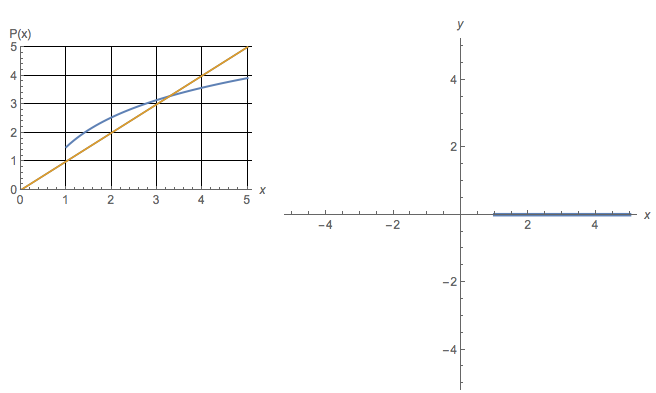
\includegraphics[width=0.8\textwidth]{img/examp2Lorenz.png} 

\subsubsection{Solution}
There's a fixed point of $P(x)$ at about $3.4$, so a closed orbit through $(3.4,0)$ is one trajectory consistent with the map.  $x = 5$ has $P(x) \approx 4$ so a trajectory that connects $(5,0)$ to $(4,0)$ (and stays outside the closed orbit) is also consistent with the map.


\subsection{identify a Hopf bifurcation point}
\subsubsection{Question}
Consider the system 
\begin{align*}
\dot x &= \mu x + y - x^3 \\
\dot y &= -x+\mu y - 2y^3.
\end{align*}

This system has a fixed point at $(0, 0)$.  For that fixed point, a Hopf bifurcation occurs at some value of $\mu$.  Identify the bifurcation value, showing your mathematical steps.


\subsubsection{Solution}
To locate the Hopf bifurcation, I want to classify the fixed point and identify when it changes stability (transitioning from a stable spiral to an unstable spiral).  At the point of bifurcation, the corresponding linear system will have a linear center.  The actual behavior of the nonlinear system is harder to determine and not something I need to figure out.

To classify the fixed point, I'll start by finding the Jacobian:

$\left(\begin{array}{c c} \mu - 3x^2 & 1 \\ -1 & \mu - 6y^2  \end{array}\right)$. At $(0,0)$, this is $\left(\begin{array}{c c} \mu  & 1 \\ -1 & \mu  \end{array}\right)$

The trace is $\tau = 2\mu$ and the determinant is $\Delta = 1+\mu^2$.  The determinant is positive for all values of $\mu$ (I need to check the sign of the determinant because when $\tau = 0$ and $\Delta < 0$ I have a saddle point, while when $\tau = 0$ and $\Delta > 0$, the linearized system has a linear center, i.e. a Hopf bifurcation).  $\tau = 0$ and $\Delta>0$ when $\mu = 0$, so the Hopf bifurcation occurs at $\mu = 0$. 


\subsection{identify bifurcations given trace and determinant information for fixed points}
\subsubsection{Question}
The plots below show the trace and determinant vs a parameter for two different fixed points that occur in a system.

Using the following graphs of the trace and determinant, classify the bifurcation(s),  identify the approximate bifurcation point(s), and identify the types of fixed points involved.

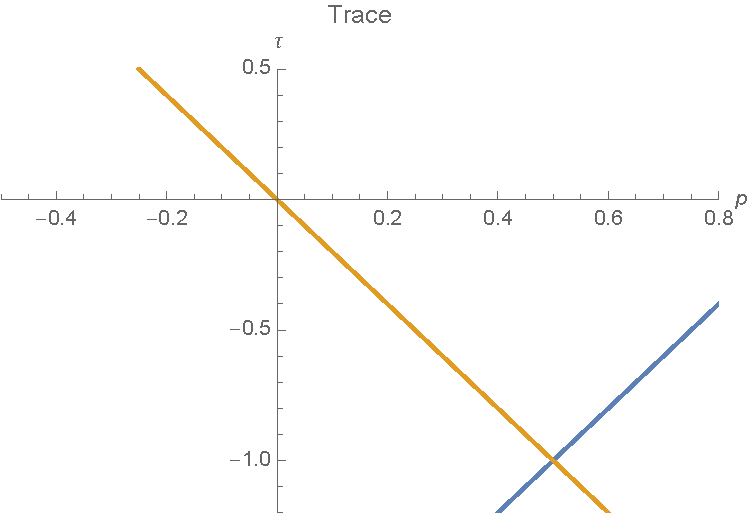
\includegraphics[width=0.4\linewidth]{img/C19-20p1a.pdf}
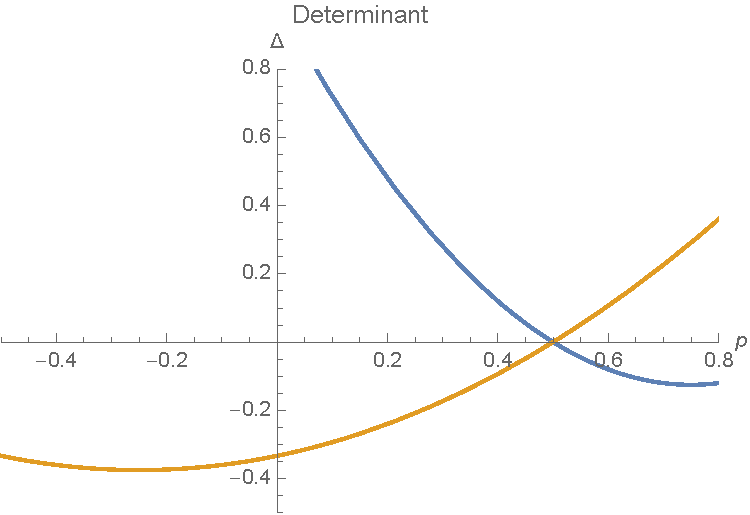
\includegraphics[width=0.4\linewidth]{img/C19-20p1b.pdf}


\subsubsection{Solution}
We are looking for parameter values when $\Delta = 0$ (for saddle-node, transcritical, pitchfork) or when $\tau = 0, \Delta>0$ (for Hopf).

The orange curve crosses $\Delta = 0$ at $p=0.5$.  When $p=0.5$, we have $\tau < 0$, so the orange fixed point transitions from a saddle point for $p<0.5$ to a stable fixed point for $p>0.5$.

The blue curve crosses $\Delta = 0$ at $p = 0.5$.  When $p=0.5$, we have $\tau<0$ so the blue fixed point transitions from stable to saddle as $p$ increases through $p=0.5$.

The orange curve crosses $\tau = 0$ at $p=0$, but $\Delta<0$, so it is not a bifurcation.

There is one bifurcation.  It involves a saddle point and a stable node exchanging stability, occurs at $p=0.5$, and is a transcritical bifurcation.



\subsection{Use phase portraits from either side of a bifurcation to identify the bifurcation}
\subsubsection{Question}
The phase portraits below are for a system on either side of a bifurcation.
\begin{itemize}
    \item For each phase portrait, fill in the chart below.
        \item Name the bifurcation.
\end{itemize}

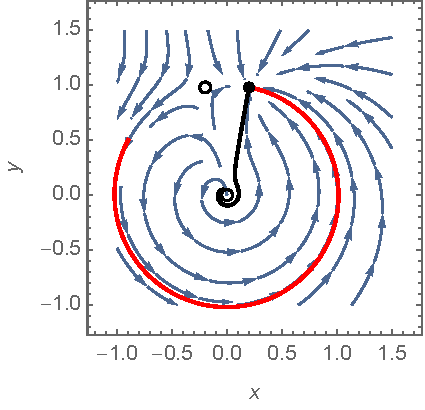
\includegraphics{img/C20-21sniperp1.pdf}
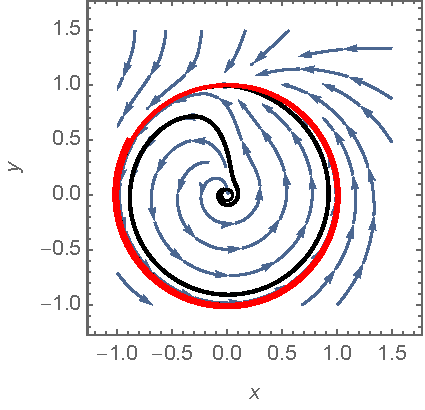
\includegraphics{img/C20-21sniperp1b.pdf}

\begin{tabular}{| c | c | c | c | c |}
\hline
plot & number of & number of  & number of  & \hspace{3in} \\
& fixed & stable & unstable &fixed point types:   \\
&  points  & limit cycles & limit cycles & attractor (a), repeller (r), or saddle (sp) \\
\hline
& & & &\\
left& & & & \\
& & & &\\
\hline
& & & &\\
right& & & & \\
& & & &\\
\hline
\end{tabular}

Name of bifurcation:



\subsubsection{Solution}

There is a repelling fixed point at the center in both phase portraits.  On the right, it looks like there is a stable limit cycle (and no other fixed points).  On the left, there is an attracting fixed point (and a saddle point).  It is not so visible, but it is there at about $(-0.2, 0.8)$ or so...  The pair of fixed points was born in a saddle-node bifurcation.

\begin{tabular}{| c | c | c | c | c |}
\hline
plot & number of & number of  & number of  & \hspace{3in} \\
& fixed & stable & unstable &fixed point types:   \\
&  points  & limit cycles & limit cycles & attractor (a), repeller (r), or saddle (sp) \\
\hline
& & & &\\
left & 3 & 0 & 0  & r,a,sp \\
& & & &\\
\hline
& & & &\\
right& 1 & 1 & 0 & r \\
& & & &\\
\hline
\end{tabular}

This is a SNIPer (saddle-node infinite period bifurcation).


\section{3d systems and maps}
\subsection{trajectory separation in a chaotic system}
\subsubsection{Question}
In the plot on the left, the $x$-coordinate is shown vs time for two trajectories of the Lorenz system.  The two trajectories started with a separation of $\delta_{old}(0) = 10^{-4}$ in their initial conditions.

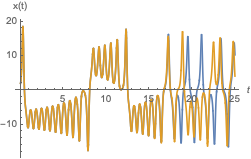
\includegraphics[width=0.45\textwidth]{img/C24-2019-11-01p1.png}\hfill
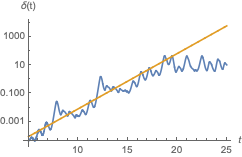
\includegraphics[width=0.45\textwidth]{img/C24-2019-11-01p2.png}

The evolution of the separation of the two trajectories, $\delta(t)$, is shown in blue on the plot on the left.  This separation grows exponentially (until it reaches approximately the size of the attractor).  A reference curve, $f(t) = ce^{0.9t}$, is plotted in orange. 


Think of the orange trajectory as the ``truth'' and the blue trajectory as a prediction.  If we'd like the prediction to be as good at time $20$ as it currently is at time $10$, how much smaller would $\delta(0)$ need to become (i.e. what is $\delta_{new}(0)$)?  As an approximation, assume $\delta(t) =\delta(0) e^{0.9t}$.

\emph{Note: $e^3\approx 20$ if you'd like to find an approximate value.}


\subsubsection{Solution}
We have $\delta(10) = \delta_{old}(0) e^{0.9*10}$.  We want $\delta(20) = \delta_{old}(0)e^{0.9*10}$ where $\delta(20) = \delta_{new}(0)e^{0.9*20}$.

$\delta_{old}(0) e^{0.9*10} = \delta_{new}(0)e^{2*0.9*10}$.

$\Rightarrow \delta_{old}(0) = \delta_{new}(0)e^{0.9*10}$ so $\delta_{new}(0) = \delta_{old}(0)*e^{-9}\approx 10^{-4}/20/20/20 = 10^{-7}/8\approx 10^{-8}$.

Four orders of magnitude smaller to double the prediction time...

\subsection{find a jacobian}
\subsubsection{Question}
Find the Jacobian for the system $\dot x = -y-z, \dot y = x + ay, \dot z = b + z(x-c).$

\subsubsection{Solution}
Finding the partials (first row is partials of $\dot x$, second row is partials of $\dot y$, and third row is partials of $\dot z$).

$\left(\begin{array}{c c c} 0 & -1 & -1 \\ 1 & a & 0 \\ z & 0 & x-c\end{array}\right)$

\subsection{use the definition of ``attractor''}
\subsubsection{Question}
Determine the attractor for the phase portrait drawn below.

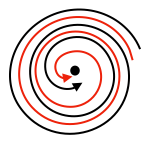
\includegraphics[]{img/C26-2019-11-06p2.png}

\subsubsection{Solution}
The stable fixed point at the center of the spirals is the only attractor visible.  It is closed, attracting, invariant, and minimal.

\subsection{applying linear stability to a period-2 orbit of a map}
\subsubsection{Question}
A map has a period-2 orbit with $1.7 = f(1.2)$ and $1.2 = f(1.7)$ with $f'(1.2) = 0.3$ and $f'(1.7) = 1.2$.

Using linear stability (so considering the  multiplier for the map $x_{n+2} = g(x_n) = f(f(x_n))$, identify the stability of the period-2 orbit.

\subsubsection{Solution}
Think of the two points in the period-$2$ orbit as $p$ and $q$, with $p = f(q)$ and $q = f(p)$

Write our map as $x_{n+2} = g(x_n)$, where our function $g$ is $f(f(x))$.  The multiplier is given by $\left.g'\right\vert_{x=q} = \left.f'(f(x))f'(x)\right\vert_{x=q}$ by the chain rule.  Substituting for $p = f(q)$ this becomes $g'(q) = f'(p)f'(q)$.  That means the stability of the 2-cycle is given by the product of the slopes at the two points involved in the 2-cycle (note that this generalizes to k-cycles...).  $f'(p) = 0.3$ and $f'(q) = 1.7$ so $g'(q) = f'(p)f'(q) = 0.3*1.7 = $ uh...

3*17 = 21+30 = 51 and I need to put in the decimals, so I get $0.51$.  That is less than $1$ in magnitude, so this 2-cycle is stable.

\subsection{count periodic orbits of a map}
\subsubsection{Question}
For the map shown below, how many period-3 orbits exist?

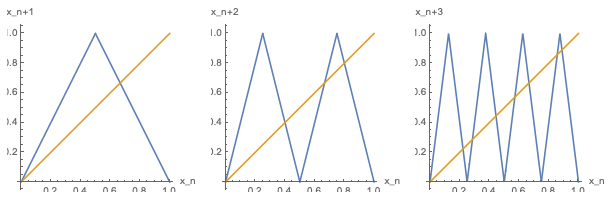
\includegraphics[width=0.9\textwidth]{img/C25-26p1a.png}


\subsubsection{Solution}
Two.

There are two period-1 points that will show up in the $x_{n+3}$ vs $x_n$ plot.  There is a period-2 orbit, but it won't show up in the $x_{n+3}$ vs $x_n$ plot.

There are eight fixed points in the $x_{n+3}$ vs $x_n$ plot.  Two of those are the period-1 points.  So six of those are period-3 points.  Six period-3 points corresponds to two period-3 orbits.

\subsection{compute similarity dimension}
\subsubsection{Question}
Recall that the similarity dimension, $d$, is given by $m = r^d$ where $r$ is a scaling factor and $m$ is the number of copies.

Find the similarity dimension for the square-based Sierpinski gasket shown below.  

\emph{The points in the set are shown in blue: you're seeing its construction through four iterates of the process.}


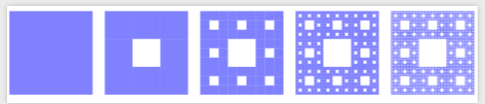
\includegraphics[width=\textwidth]{img/C29-2019-11-13p2.png}

\subsubsection{Solution}

\begin{tabular}{|c|p{3cm}|}
\hline
scaling factor: & $r = 3$ \\
\hline
copies: & $m=8$ \\
\hline
dimension: & $d=\ln 8/\ln 3$ \\
\hline
\end{tabular}


\vspace{0.1cm}

From the left image to the second image, each side of the large square scales down by a factor of three, and then we make eight copies (we are leaving the center one out).  So the dimension should be almost $2$, but not quite.

$8 = 3^d$ so $d = \ln 8/\ln 3 \approx 1.89$.

\subsection{identify a periodic window for the logistic map from an orbit diagram}
\subsubsection{Question}
The image below is an excerpt of the orbit diagram for the logistic map, given by $x_{n+1} = f(x_n)$ for $f(x) = rx(1-x).$

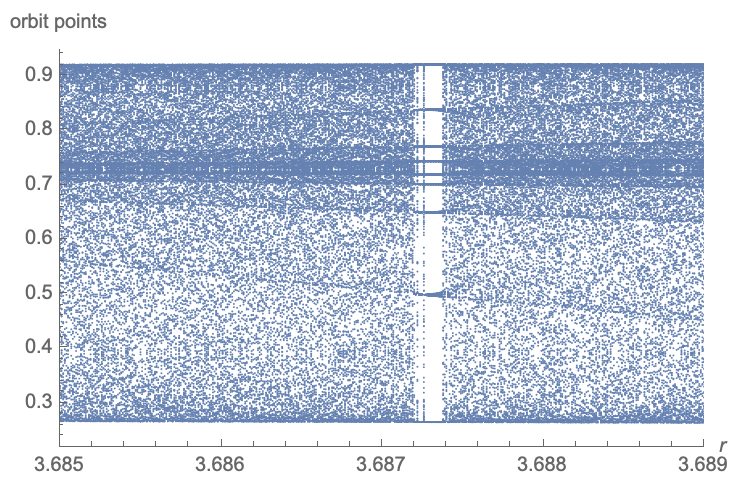
\includegraphics{img/C28-2019-11-11p2.png}

There is a very visible ``periodic window'' in the map.  Within the window, a number of different periods of periodic orbit occur.

\begin{itemize}
    \item Identify the lowest period of periodic orbit visible in the window.
    \item Provide an estimate of a parameter value where that period of orbit is occurring.
    \item The periodic orbit you identified above would manifest as $k$ (stable) fixed points in some map.  Provide an expression for that map.
\end{itemize}  

\subsubsection{Solution}
There's a clear periodic window at around $p = 3.6873$ or so.

I see nine somewhat horizontal lines in the window, so the lowest period visible in there is nine points (there are going to be period-doubling bifurcations within the window: 9 to 18 to 36 to etc, in a period-doubling cascade, but 9 is the lowest).

These nine points will be nine fixed points of $f^9(x)$ (period-1 and period-3 points will also be fixed points of that map.)

\subsection{calculating using a functional equation}
\subsubsection{Question}
Consider the functional equation $f(xy) = f(x) + f(y)$.  Use $1 = 1*1$ to find a value for $f(1)$.

\subsubsection{Solution}
We have $f(1) = f(1*1) = f(1)+f(1) = 2f(1)$ so $f(1) = 2f(1) \Rightarrow f(1) = 0$.

\subsection{identify a superstable fixed point}
\subsubsection{Question}
Consider the map $x_{n+1} = r\sin x_n$ with $0\leq x \leq \pi$.  Find $x^*$ and $r_0$ such that $x^*$ is a superstable fixed point of the map at $r = r_0$.

\subsubsection{Solution}
At a superstable fixed point, $f'(x) = 0$.  $f(x) = r\sin x$ and $f'(x) = r\cos x$.  For $x \in [0,\pi]$, $\cos x = 0$ when $x = \pi/2$.  We want $x^* = \pi/2$ to be a fixed point of the map (in order to have a superstable fixed point).  We have $\pi/2 = r_0\sin\pi/2 = r$, so $r_0 = \pi/2$.  


\end{document}